% Created by tikzDevice version 0.12.3.1 on 2022-02-28 16:49:08
% !TEX encoding = UTF-8 Unicode
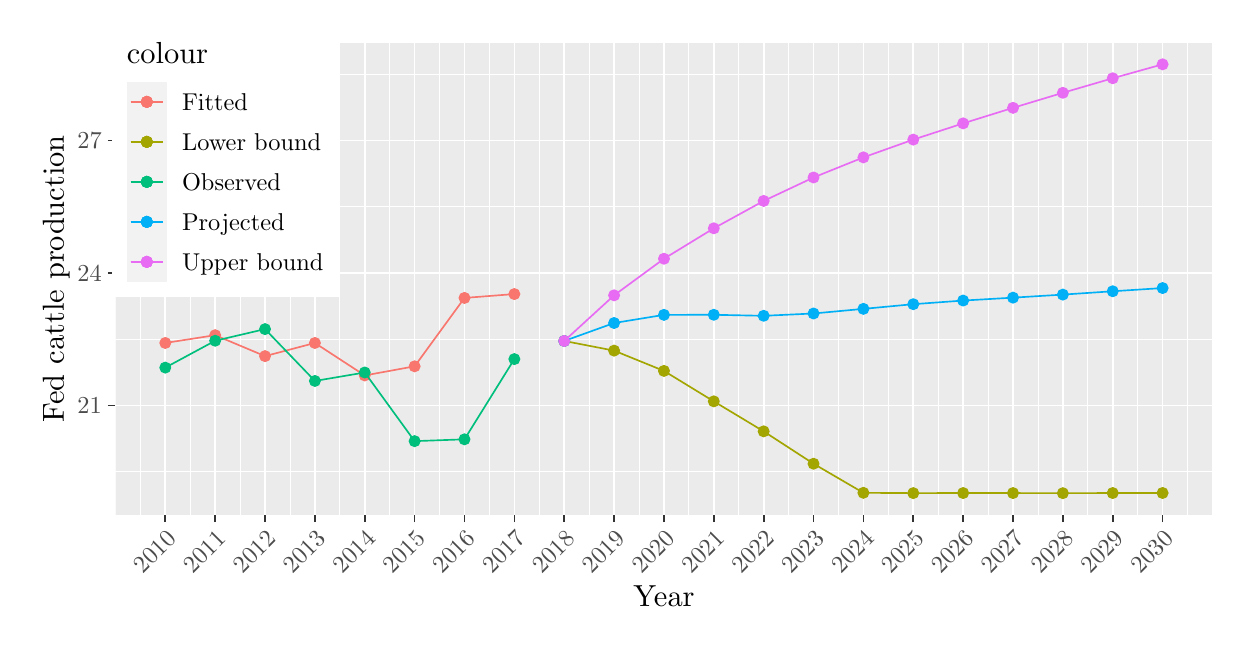
\begin{tikzpicture}[x=1pt,y=1pt]
\definecolor{fillColor}{RGB}{255,255,255}
\path[use as bounding box,fill=fillColor,fill opacity=0.00] (0,0) rectangle (433.62,216.81);
\begin{scope}
\path[clip] (  0.00,  0.00) rectangle (433.62,216.81);
\definecolor{drawColor}{RGB}{255,255,255}
\definecolor{fillColor}{RGB}{255,255,255}

\path[draw=drawColor,line width= 0.6pt,line join=round,line cap=round,fill=fillColor] (  0.00,  0.00) rectangle (433.62,216.81);
\end{scope}
\begin{scope}
\path[clip] ( 31.71, 40.85) rectangle (428.12,211.31);
\definecolor{fillColor}{gray}{0.92}

\path[fill=fillColor] ( 31.71, 40.85) rectangle (428.12,211.31);
\definecolor{drawColor}{RGB}{255,255,255}

\path[draw=drawColor,line width= 0.3pt,line join=round] ( 31.71, 56.41) --
	(428.12, 56.41);

\path[draw=drawColor,line width= 0.3pt,line join=round] ( 31.71,104.28) --
	(428.12,104.28);

\path[draw=drawColor,line width= 0.3pt,line join=round] ( 31.71,152.14) --
	(428.12,152.14);

\path[draw=drawColor,line width= 0.3pt,line join=round] ( 31.71,200.01) --
	(428.12,200.01);

\path[draw=drawColor,line width= 0.3pt,line join=round] ( 31.71, 40.85) --
	( 31.71,211.31);

\path[draw=drawColor,line width= 0.3pt,line join=round] ( 40.72, 40.85) --
	( 40.72,211.31);

\path[draw=drawColor,line width= 0.3pt,line join=round] ( 58.74, 40.85) --
	( 58.74,211.31);

\path[draw=drawColor,line width= 0.3pt,line join=round] ( 76.76, 40.85) --
	( 76.76,211.31);

\path[draw=drawColor,line width= 0.3pt,line join=round] ( 94.78, 40.85) --
	( 94.78,211.31);

\path[draw=drawColor,line width= 0.3pt,line join=round] (112.80, 40.85) --
	(112.80,211.31);

\path[draw=drawColor,line width= 0.3pt,line join=round] (130.81, 40.85) --
	(130.81,211.31);

\path[draw=drawColor,line width= 0.3pt,line join=round] (148.83, 40.85) --
	(148.83,211.31);

\path[draw=drawColor,line width= 0.3pt,line join=round] (166.85, 40.85) --
	(166.85,211.31);

\path[draw=drawColor,line width= 0.3pt,line join=round] (184.87, 40.85) --
	(184.87,211.31);

\path[draw=drawColor,line width= 0.3pt,line join=round] (202.89, 40.85) --
	(202.89,211.31);

\path[draw=drawColor,line width= 0.3pt,line join=round] (220.91, 40.85) --
	(220.91,211.31);

\path[draw=drawColor,line width= 0.3pt,line join=round] (238.93, 40.85) --
	(238.93,211.31);

\path[draw=drawColor,line width= 0.3pt,line join=round] (256.94, 40.85) --
	(256.94,211.31);

\path[draw=drawColor,line width= 0.3pt,line join=round] (274.96, 40.85) --
	(274.96,211.31);

\path[draw=drawColor,line width= 0.3pt,line join=round] (292.98, 40.85) --
	(292.98,211.31);

\path[draw=drawColor,line width= 0.3pt,line join=round] (311.00, 40.85) --
	(311.00,211.31);

\path[draw=drawColor,line width= 0.3pt,line join=round] (329.02, 40.85) --
	(329.02,211.31);

\path[draw=drawColor,line width= 0.3pt,line join=round] (347.04, 40.85) --
	(347.04,211.31);

\path[draw=drawColor,line width= 0.3pt,line join=round] (365.06, 40.85) --
	(365.06,211.31);

\path[draw=drawColor,line width= 0.3pt,line join=round] (383.07, 40.85) --
	(383.07,211.31);

\path[draw=drawColor,line width= 0.3pt,line join=round] (401.09, 40.85) --
	(401.09,211.31);

\path[draw=drawColor,line width= 0.3pt,line join=round] (419.11, 40.85) --
	(419.11,211.31);

\path[draw=drawColor,line width= 0.3pt,line join=round] (428.12, 40.85) --
	(428.12,211.31);

\path[draw=drawColor,line width= 0.6pt,line join=round] ( 31.71, 80.34) --
	(428.12, 80.34);

\path[draw=drawColor,line width= 0.6pt,line join=round] ( 31.71,128.21) --
	(428.12,128.21);

\path[draw=drawColor,line width= 0.6pt,line join=round] ( 31.71,176.08) --
	(428.12,176.08);

\path[draw=drawColor,line width= 0.6pt,line join=round] ( 49.73, 40.85) --
	( 49.73,211.31);

\path[draw=drawColor,line width= 0.6pt,line join=round] ( 67.75, 40.85) --
	( 67.75,211.31);

\path[draw=drawColor,line width= 0.6pt,line join=round] ( 85.77, 40.85) --
	( 85.77,211.31);

\path[draw=drawColor,line width= 0.6pt,line join=round] (103.79, 40.85) --
	(103.79,211.31);

\path[draw=drawColor,line width= 0.6pt,line join=round] (121.80, 40.85) --
	(121.80,211.31);

\path[draw=drawColor,line width= 0.6pt,line join=round] (139.82, 40.85) --
	(139.82,211.31);

\path[draw=drawColor,line width= 0.6pt,line join=round] (157.84, 40.85) --
	(157.84,211.31);

\path[draw=drawColor,line width= 0.6pt,line join=round] (175.86, 40.85) --
	(175.86,211.31);

\path[draw=drawColor,line width= 0.6pt,line join=round] (193.88, 40.85) --
	(193.88,211.31);

\path[draw=drawColor,line width= 0.6pt,line join=round] (211.90, 40.85) --
	(211.90,211.31);

\path[draw=drawColor,line width= 0.6pt,line join=round] (229.92, 40.85) --
	(229.92,211.31);

\path[draw=drawColor,line width= 0.6pt,line join=round] (247.93, 40.85) --
	(247.93,211.31);

\path[draw=drawColor,line width= 0.6pt,line join=round] (265.95, 40.85) --
	(265.95,211.31);

\path[draw=drawColor,line width= 0.6pt,line join=round] (283.97, 40.85) --
	(283.97,211.31);

\path[draw=drawColor,line width= 0.6pt,line join=round] (301.99, 40.85) --
	(301.99,211.31);

\path[draw=drawColor,line width= 0.6pt,line join=round] (320.01, 40.85) --
	(320.01,211.31);

\path[draw=drawColor,line width= 0.6pt,line join=round] (338.03, 40.85) --
	(338.03,211.31);

\path[draw=drawColor,line width= 0.6pt,line join=round] (356.05, 40.85) --
	(356.05,211.31);

\path[draw=drawColor,line width= 0.6pt,line join=round] (374.06, 40.85) --
	(374.06,211.31);

\path[draw=drawColor,line width= 0.6pt,line join=round] (392.08, 40.85) --
	(392.08,211.31);

\path[draw=drawColor,line width= 0.6pt,line join=round] (410.10, 40.85) --
	(410.10,211.31);
\definecolor{drawColor}{RGB}{248,118,109}

\path[draw=drawColor,line width= 0.6pt,line join=round] ( 49.73,102.88) --
	( 67.75,105.69) --
	( 85.77, 98.12) --
	(103.79,102.88) --
	(121.80, 91.14) --
	(139.82, 94.44) --
	(157.84,119.15) --
	(175.86,120.55);
\definecolor{fillColor}{RGB}{248,118,109}

\path[draw=drawColor,line width= 0.4pt,line join=round,line cap=round,fill=fillColor] ( 49.73,102.88) circle (  1.96);

\path[draw=drawColor,line width= 0.4pt,line join=round,line cap=round,fill=fillColor] ( 67.75,105.69) circle (  1.96);

\path[draw=drawColor,line width= 0.4pt,line join=round,line cap=round,fill=fillColor] ( 85.77, 98.12) circle (  1.96);

\path[draw=drawColor,line width= 0.4pt,line join=round,line cap=round,fill=fillColor] (103.79,102.88) circle (  1.96);

\path[draw=drawColor,line width= 0.4pt,line join=round,line cap=round,fill=fillColor] (121.80, 91.14) circle (  1.96);

\path[draw=drawColor,line width= 0.4pt,line join=round,line cap=round,fill=fillColor] (139.82, 94.44) circle (  1.96);

\path[draw=drawColor,line width= 0.4pt,line join=round,line cap=round,fill=fillColor] (157.84,119.15) circle (  1.96);

\path[draw=drawColor,line width= 0.4pt,line join=round,line cap=round,fill=fillColor] (175.86,120.55) circle (  1.96);
\definecolor{drawColor}{RGB}{0,191,125}

\path[draw=drawColor,line width= 0.6pt,line join=round] ( 49.73, 93.97) --
	( 67.75,103.68) --
	( 85.77,107.88) --
	(103.79, 89.15) --
	(121.80, 92.21) --
	(139.82, 67.40) --
	(157.84, 68.06) --
	(175.86, 97.05);
\definecolor{fillColor}{RGB}{0,191,125}

\path[draw=drawColor,line width= 0.4pt,line join=round,line cap=round,fill=fillColor] ( 49.73, 93.97) circle (  1.96);

\path[draw=drawColor,line width= 0.4pt,line join=round,line cap=round,fill=fillColor] ( 67.75,103.68) circle (  1.96);

\path[draw=drawColor,line width= 0.4pt,line join=round,line cap=round,fill=fillColor] ( 85.77,107.88) circle (  1.96);

\path[draw=drawColor,line width= 0.4pt,line join=round,line cap=round,fill=fillColor] (103.79, 89.15) circle (  1.96);

\path[draw=drawColor,line width= 0.4pt,line join=round,line cap=round,fill=fillColor] (121.80, 92.21) circle (  1.96);

\path[draw=drawColor,line width= 0.4pt,line join=round,line cap=round,fill=fillColor] (139.82, 67.40) circle (  1.96);

\path[draw=drawColor,line width= 0.4pt,line join=round,line cap=round,fill=fillColor] (157.84, 68.06) circle (  1.96);

\path[draw=drawColor,line width= 0.4pt,line join=round,line cap=round,fill=fillColor] (175.86, 97.05) circle (  1.96);
\definecolor{drawColor}{RGB}{163,165,0}

\path[draw=drawColor,line width= 0.6pt,line join=round] (193.88,103.60) --
	(211.90,100.11) --
	(229.92, 92.78) --
	(247.93, 81.78) --
	(265.95, 70.94) --
	(283.97, 59.24) --
	(301.99, 48.73) --
	(320.01, 48.62) --
	(338.03, 48.65) --
	(356.05, 48.64) --
	(374.06, 48.60) --
	(392.08, 48.65) --
	(410.10, 48.67);
\definecolor{fillColor}{RGB}{163,165,0}

\path[draw=drawColor,line width= 0.4pt,line join=round,line cap=round,fill=fillColor] (193.88,103.60) circle (  1.96);

\path[draw=drawColor,line width= 0.4pt,line join=round,line cap=round,fill=fillColor] (211.90,100.11) circle (  1.96);

\path[draw=drawColor,line width= 0.4pt,line join=round,line cap=round,fill=fillColor] (229.92, 92.78) circle (  1.96);

\path[draw=drawColor,line width= 0.4pt,line join=round,line cap=round,fill=fillColor] (247.93, 81.78) circle (  1.96);

\path[draw=drawColor,line width= 0.4pt,line join=round,line cap=round,fill=fillColor] (265.95, 70.94) circle (  1.96);

\path[draw=drawColor,line width= 0.4pt,line join=round,line cap=round,fill=fillColor] (283.97, 59.24) circle (  1.96);

\path[draw=drawColor,line width= 0.4pt,line join=round,line cap=round,fill=fillColor] (301.99, 48.73) circle (  1.96);

\path[draw=drawColor,line width= 0.4pt,line join=round,line cap=round,fill=fillColor] (320.01, 48.62) circle (  1.96);

\path[draw=drawColor,line width= 0.4pt,line join=round,line cap=round,fill=fillColor] (338.03, 48.65) circle (  1.96);

\path[draw=drawColor,line width= 0.4pt,line join=round,line cap=round,fill=fillColor] (356.05, 48.64) circle (  1.96);

\path[draw=drawColor,line width= 0.4pt,line join=round,line cap=round,fill=fillColor] (374.06, 48.60) circle (  1.96);

\path[draw=drawColor,line width= 0.4pt,line join=round,line cap=round,fill=fillColor] (392.08, 48.65) circle (  1.96);

\path[draw=drawColor,line width= 0.4pt,line join=round,line cap=round,fill=fillColor] (410.10, 48.67) circle (  1.96);
\definecolor{drawColor}{RGB}{0,176,246}

\path[draw=drawColor,line width= 0.6pt,line join=round] (193.88,103.60) --
	(211.90,110.09) --
	(229.92,113.03) --
	(247.93,113.06) --
	(265.95,112.69) --
	(283.97,113.53) --
	(301.99,115.20) --
	(320.01,116.89) --
	(338.03,118.20) --
	(356.05,119.25) --
	(374.06,120.35) --
	(392.08,121.56) --
	(410.10,122.72);
\definecolor{fillColor}{RGB}{0,176,246}

\path[draw=drawColor,line width= 0.4pt,line join=round,line cap=round,fill=fillColor] (193.88,103.60) circle (  1.96);

\path[draw=drawColor,line width= 0.4pt,line join=round,line cap=round,fill=fillColor] (211.90,110.09) circle (  1.96);

\path[draw=drawColor,line width= 0.4pt,line join=round,line cap=round,fill=fillColor] (229.92,113.03) circle (  1.96);

\path[draw=drawColor,line width= 0.4pt,line join=round,line cap=round,fill=fillColor] (247.93,113.06) circle (  1.96);

\path[draw=drawColor,line width= 0.4pt,line join=round,line cap=round,fill=fillColor] (265.95,112.69) circle (  1.96);

\path[draw=drawColor,line width= 0.4pt,line join=round,line cap=round,fill=fillColor] (283.97,113.53) circle (  1.96);

\path[draw=drawColor,line width= 0.4pt,line join=round,line cap=round,fill=fillColor] (301.99,115.20) circle (  1.96);

\path[draw=drawColor,line width= 0.4pt,line join=round,line cap=round,fill=fillColor] (320.01,116.89) circle (  1.96);

\path[draw=drawColor,line width= 0.4pt,line join=round,line cap=round,fill=fillColor] (338.03,118.20) circle (  1.96);

\path[draw=drawColor,line width= 0.4pt,line join=round,line cap=round,fill=fillColor] (356.05,119.25) circle (  1.96);

\path[draw=drawColor,line width= 0.4pt,line join=round,line cap=round,fill=fillColor] (374.06,120.35) circle (  1.96);

\path[draw=drawColor,line width= 0.4pt,line join=round,line cap=round,fill=fillColor] (392.08,121.56) circle (  1.96);

\path[draw=drawColor,line width= 0.4pt,line join=round,line cap=round,fill=fillColor] (410.10,122.72) circle (  1.96);
\definecolor{drawColor}{RGB}{231,107,243}

\path[draw=drawColor,line width= 0.6pt,line join=round] (193.88,103.60) --
	(211.90,120.09) --
	(229.92,133.31) --
	(247.93,144.31) --
	(265.95,154.20) --
	(283.97,162.68) --
	(301.99,169.94) --
	(320.01,176.36) --
	(338.03,182.23) --
	(356.05,187.84) --
	(374.06,193.27) --
	(392.08,198.53) --
	(410.10,203.56);
\definecolor{fillColor}{RGB}{231,107,243}

\path[draw=drawColor,line width= 0.4pt,line join=round,line cap=round,fill=fillColor] (193.88,103.60) circle (  1.96);

\path[draw=drawColor,line width= 0.4pt,line join=round,line cap=round,fill=fillColor] (211.90,120.09) circle (  1.96);

\path[draw=drawColor,line width= 0.4pt,line join=round,line cap=round,fill=fillColor] (229.92,133.31) circle (  1.96);

\path[draw=drawColor,line width= 0.4pt,line join=round,line cap=round,fill=fillColor] (247.93,144.31) circle (  1.96);

\path[draw=drawColor,line width= 0.4pt,line join=round,line cap=round,fill=fillColor] (265.95,154.20) circle (  1.96);

\path[draw=drawColor,line width= 0.4pt,line join=round,line cap=round,fill=fillColor] (283.97,162.68) circle (  1.96);

\path[draw=drawColor,line width= 0.4pt,line join=round,line cap=round,fill=fillColor] (301.99,169.94) circle (  1.96);

\path[draw=drawColor,line width= 0.4pt,line join=round,line cap=round,fill=fillColor] (320.01,176.36) circle (  1.96);

\path[draw=drawColor,line width= 0.4pt,line join=round,line cap=round,fill=fillColor] (338.03,182.23) circle (  1.96);

\path[draw=drawColor,line width= 0.4pt,line join=round,line cap=round,fill=fillColor] (356.05,187.84) circle (  1.96);

\path[draw=drawColor,line width= 0.4pt,line join=round,line cap=round,fill=fillColor] (374.06,193.27) circle (  1.96);

\path[draw=drawColor,line width= 0.4pt,line join=round,line cap=round,fill=fillColor] (392.08,198.53) circle (  1.96);

\path[draw=drawColor,line width= 0.4pt,line join=round,line cap=round,fill=fillColor] (410.10,203.56) circle (  1.96);
\end{scope}
\begin{scope}
\path[clip] (  0.00,  0.00) rectangle (433.62,216.81);
\definecolor{drawColor}{gray}{0.30}

\node[text=drawColor,anchor=base east,inner sep=0pt, outer sep=0pt, scale=  0.88] at ( 26.76, 77.31) {21};

\node[text=drawColor,anchor=base east,inner sep=0pt, outer sep=0pt, scale=  0.88] at ( 26.76,125.18) {24};

\node[text=drawColor,anchor=base east,inner sep=0pt, outer sep=0pt, scale=  0.88] at ( 26.76,173.05) {27};
\end{scope}
\begin{scope}
\path[clip] (  0.00,  0.00) rectangle (433.62,216.81);
\definecolor{drawColor}{gray}{0.20}

\path[draw=drawColor,line width= 0.6pt,line join=round] ( 28.96, 80.34) --
	( 31.71, 80.34);

\path[draw=drawColor,line width= 0.6pt,line join=round] ( 28.96,128.21) --
	( 31.71,128.21);

\path[draw=drawColor,line width= 0.6pt,line join=round] ( 28.96,176.08) --
	( 31.71,176.08);
\end{scope}
\begin{scope}
\path[clip] (  0.00,  0.00) rectangle (433.62,216.81);
\definecolor{drawColor}{gray}{0.20}

\path[draw=drawColor,line width= 0.6pt,line join=round] ( 49.73, 38.10) --
	( 49.73, 40.85);

\path[draw=drawColor,line width= 0.6pt,line join=round] ( 67.75, 38.10) --
	( 67.75, 40.85);

\path[draw=drawColor,line width= 0.6pt,line join=round] ( 85.77, 38.10) --
	( 85.77, 40.85);

\path[draw=drawColor,line width= 0.6pt,line join=round] (103.79, 38.10) --
	(103.79, 40.85);

\path[draw=drawColor,line width= 0.6pt,line join=round] (121.80, 38.10) --
	(121.80, 40.85);

\path[draw=drawColor,line width= 0.6pt,line join=round] (139.82, 38.10) --
	(139.82, 40.85);

\path[draw=drawColor,line width= 0.6pt,line join=round] (157.84, 38.10) --
	(157.84, 40.85);

\path[draw=drawColor,line width= 0.6pt,line join=round] (175.86, 38.10) --
	(175.86, 40.85);

\path[draw=drawColor,line width= 0.6pt,line join=round] (193.88, 38.10) --
	(193.88, 40.85);

\path[draw=drawColor,line width= 0.6pt,line join=round] (211.90, 38.10) --
	(211.90, 40.85);

\path[draw=drawColor,line width= 0.6pt,line join=round] (229.92, 38.10) --
	(229.92, 40.85);

\path[draw=drawColor,line width= 0.6pt,line join=round] (247.93, 38.10) --
	(247.93, 40.85);

\path[draw=drawColor,line width= 0.6pt,line join=round] (265.95, 38.10) --
	(265.95, 40.85);

\path[draw=drawColor,line width= 0.6pt,line join=round] (283.97, 38.10) --
	(283.97, 40.85);

\path[draw=drawColor,line width= 0.6pt,line join=round] (301.99, 38.10) --
	(301.99, 40.85);

\path[draw=drawColor,line width= 0.6pt,line join=round] (320.01, 38.10) --
	(320.01, 40.85);

\path[draw=drawColor,line width= 0.6pt,line join=round] (338.03, 38.10) --
	(338.03, 40.85);

\path[draw=drawColor,line width= 0.6pt,line join=round] (356.05, 38.10) --
	(356.05, 40.85);

\path[draw=drawColor,line width= 0.6pt,line join=round] (374.06, 38.10) --
	(374.06, 40.85);

\path[draw=drawColor,line width= 0.6pt,line join=round] (392.08, 38.10) --
	(392.08, 40.85);

\path[draw=drawColor,line width= 0.6pt,line join=round] (410.10, 38.10) --
	(410.10, 40.85);
\end{scope}
\begin{scope}
\path[clip] (  0.00,  0.00) rectangle (433.62,216.81);
\definecolor{drawColor}{gray}{0.30}

\node[text=drawColor,rotate= 45.00,anchor=base east,inner sep=0pt, outer sep=0pt, scale=  0.88] at ( 54.02, 31.62) {2010};

\node[text=drawColor,rotate= 45.00,anchor=base east,inner sep=0pt, outer sep=0pt, scale=  0.88] at ( 72.03, 31.62) {2011};

\node[text=drawColor,rotate= 45.00,anchor=base east,inner sep=0pt, outer sep=0pt, scale=  0.88] at ( 90.05, 31.62) {2012};

\node[text=drawColor,rotate= 45.00,anchor=base east,inner sep=0pt, outer sep=0pt, scale=  0.88] at (108.07, 31.62) {2013};

\node[text=drawColor,rotate= 45.00,anchor=base east,inner sep=0pt, outer sep=0pt, scale=  0.88] at (126.09, 31.62) {2014};

\node[text=drawColor,rotate= 45.00,anchor=base east,inner sep=0pt, outer sep=0pt, scale=  0.88] at (144.11, 31.62) {2015};

\node[text=drawColor,rotate= 45.00,anchor=base east,inner sep=0pt, outer sep=0pt, scale=  0.88] at (162.13, 31.62) {2016};

\node[text=drawColor,rotate= 45.00,anchor=base east,inner sep=0pt, outer sep=0pt, scale=  0.88] at (180.15, 31.62) {2017};

\node[text=drawColor,rotate= 45.00,anchor=base east,inner sep=0pt, outer sep=0pt, scale=  0.88] at (198.16, 31.62) {2018};

\node[text=drawColor,rotate= 45.00,anchor=base east,inner sep=0pt, outer sep=0pt, scale=  0.88] at (216.18, 31.62) {2019};

\node[text=drawColor,rotate= 45.00,anchor=base east,inner sep=0pt, outer sep=0pt, scale=  0.88] at (234.20, 31.62) {2020};

\node[text=drawColor,rotate= 45.00,anchor=base east,inner sep=0pt, outer sep=0pt, scale=  0.88] at (252.22, 31.62) {2021};

\node[text=drawColor,rotate= 45.00,anchor=base east,inner sep=0pt, outer sep=0pt, scale=  0.88] at (270.24, 31.62) {2022};

\node[text=drawColor,rotate= 45.00,anchor=base east,inner sep=0pt, outer sep=0pt, scale=  0.88] at (288.26, 31.62) {2023};

\node[text=drawColor,rotate= 45.00,anchor=base east,inner sep=0pt, outer sep=0pt, scale=  0.88] at (306.28, 31.62) {2024};

\node[text=drawColor,rotate= 45.00,anchor=base east,inner sep=0pt, outer sep=0pt, scale=  0.88] at (324.29, 31.62) {2025};

\node[text=drawColor,rotate= 45.00,anchor=base east,inner sep=0pt, outer sep=0pt, scale=  0.88] at (342.31, 31.62) {2026};

\node[text=drawColor,rotate= 45.00,anchor=base east,inner sep=0pt, outer sep=0pt, scale=  0.88] at (360.33, 31.62) {2027};

\node[text=drawColor,rotate= 45.00,anchor=base east,inner sep=0pt, outer sep=0pt, scale=  0.88] at (378.35, 31.62) {2028};

\node[text=drawColor,rotate= 45.00,anchor=base east,inner sep=0pt, outer sep=0pt, scale=  0.88] at (396.37, 31.62) {2029};

\node[text=drawColor,rotate= 45.00,anchor=base east,inner sep=0pt, outer sep=0pt, scale=  0.88] at (414.39, 31.62) {2030};
\end{scope}
\begin{scope}
\path[clip] (  0.00,  0.00) rectangle (433.62,216.81);
\definecolor{drawColor}{RGB}{0,0,0}

\node[text=drawColor,anchor=base,inner sep=0pt, outer sep=0pt, scale=  1.10] at (229.92,  7.64) {Year};
\end{scope}
\begin{scope}
\path[clip] (  0.00,  0.00) rectangle (433.62,216.81);
\definecolor{drawColor}{RGB}{0,0,0}

\node[text=drawColor,rotate= 90.00,anchor=base,inner sep=0pt, outer sep=0pt, scale=  1.10] at ( 13.08,126.08) {Fed cattle production};
\end{scope}
\begin{scope}
\path[clip] (  0.00,  0.00) rectangle (433.62,216.81);
\definecolor{fillColor}{RGB}{255,255,255}

\path[fill=fillColor] ( 30.33,119.45) rectangle (112.38,217.94);
\end{scope}
\begin{scope}
\path[clip] (  0.00,  0.00) rectangle (433.62,216.81);
\definecolor{drawColor}{RGB}{0,0,0}

\node[text=drawColor,anchor=base west,inner sep=0pt, outer sep=0pt, scale=  1.10] at ( 35.83,203.79) {colour};
\end{scope}
\begin{scope}
\path[clip] (  0.00,  0.00) rectangle (433.62,216.81);
\definecolor{fillColor}{gray}{0.95}

\path[fill=fillColor] ( 35.83,182.77) rectangle ( 50.28,197.22);
\end{scope}
\begin{scope}
\path[clip] (  0.00,  0.00) rectangle (433.62,216.81);
\definecolor{drawColor}{RGB}{248,118,109}

\path[draw=drawColor,line width= 0.6pt,line join=round] ( 37.27,190.00) -- ( 48.83,190.00);
\end{scope}
\begin{scope}
\path[clip] (  0.00,  0.00) rectangle (433.62,216.81);
\definecolor{drawColor}{RGB}{248,118,109}
\definecolor{fillColor}{RGB}{248,118,109}

\path[draw=drawColor,line width= 0.4pt,line join=round,line cap=round,fill=fillColor] ( 43.05,190.00) circle (  1.96);
\end{scope}
\begin{scope}
\path[clip] (  0.00,  0.00) rectangle (433.62,216.81);
\definecolor{drawColor}{RGB}{248,118,109}

\path[draw=drawColor,line width= 0.6pt,line join=round] ( 37.27,190.00) -- ( 48.83,190.00);
\end{scope}
\begin{scope}
\path[clip] (  0.00,  0.00) rectangle (433.62,216.81);
\definecolor{drawColor}{RGB}{248,118,109}
\definecolor{fillColor}{RGB}{248,118,109}

\path[draw=drawColor,line width= 0.4pt,line join=round,line cap=round,fill=fillColor] ( 43.05,190.00) circle (  1.96);
\end{scope}
\begin{scope}
\path[clip] (  0.00,  0.00) rectangle (433.62,216.81);
\definecolor{drawColor}{RGB}{248,118,109}

\path[draw=drawColor,line width= 0.6pt,line join=round] ( 37.27,190.00) -- ( 48.83,190.00);
\end{scope}
\begin{scope}
\path[clip] (  0.00,  0.00) rectangle (433.62,216.81);
\definecolor{drawColor}{RGB}{248,118,109}
\definecolor{fillColor}{RGB}{248,118,109}

\path[draw=drawColor,line width= 0.4pt,line join=round,line cap=round,fill=fillColor] ( 43.05,190.00) circle (  1.96);
\end{scope}
\begin{scope}
\path[clip] (  0.00,  0.00) rectangle (433.62,216.81);
\definecolor{drawColor}{RGB}{248,118,109}

\path[draw=drawColor,line width= 0.6pt,line join=round] ( 37.27,190.00) -- ( 48.83,190.00);
\end{scope}
\begin{scope}
\path[clip] (  0.00,  0.00) rectangle (433.62,216.81);
\definecolor{drawColor}{RGB}{248,118,109}
\definecolor{fillColor}{RGB}{248,118,109}

\path[draw=drawColor,line width= 0.4pt,line join=round,line cap=round,fill=fillColor] ( 43.05,190.00) circle (  1.96);
\end{scope}
\begin{scope}
\path[clip] (  0.00,  0.00) rectangle (433.62,216.81);
\definecolor{drawColor}{RGB}{248,118,109}

\path[draw=drawColor,line width= 0.6pt,line join=round] ( 37.27,190.00) -- ( 48.83,190.00);
\end{scope}
\begin{scope}
\path[clip] (  0.00,  0.00) rectangle (433.62,216.81);
\definecolor{drawColor}{RGB}{248,118,109}
\definecolor{fillColor}{RGB}{248,118,109}

\path[draw=drawColor,line width= 0.4pt,line join=round,line cap=round,fill=fillColor] ( 43.05,190.00) circle (  1.96);
\end{scope}
\begin{scope}
\path[clip] (  0.00,  0.00) rectangle (433.62,216.81);
\definecolor{fillColor}{gray}{0.95}

\path[fill=fillColor] ( 35.83,168.32) rectangle ( 50.28,182.77);
\end{scope}
\begin{scope}
\path[clip] (  0.00,  0.00) rectangle (433.62,216.81);
\definecolor{drawColor}{RGB}{163,165,0}

\path[draw=drawColor,line width= 0.6pt,line join=round] ( 37.27,175.54) -- ( 48.83,175.54);
\end{scope}
\begin{scope}
\path[clip] (  0.00,  0.00) rectangle (433.62,216.81);
\definecolor{drawColor}{RGB}{163,165,0}
\definecolor{fillColor}{RGB}{163,165,0}

\path[draw=drawColor,line width= 0.4pt,line join=round,line cap=round,fill=fillColor] ( 43.05,175.54) circle (  1.96);
\end{scope}
\begin{scope}
\path[clip] (  0.00,  0.00) rectangle (433.62,216.81);
\definecolor{drawColor}{RGB}{163,165,0}

\path[draw=drawColor,line width= 0.6pt,line join=round] ( 37.27,175.54) -- ( 48.83,175.54);
\end{scope}
\begin{scope}
\path[clip] (  0.00,  0.00) rectangle (433.62,216.81);
\definecolor{drawColor}{RGB}{163,165,0}
\definecolor{fillColor}{RGB}{163,165,0}

\path[draw=drawColor,line width= 0.4pt,line join=round,line cap=round,fill=fillColor] ( 43.05,175.54) circle (  1.96);
\end{scope}
\begin{scope}
\path[clip] (  0.00,  0.00) rectangle (433.62,216.81);
\definecolor{drawColor}{RGB}{163,165,0}

\path[draw=drawColor,line width= 0.6pt,line join=round] ( 37.27,175.54) -- ( 48.83,175.54);
\end{scope}
\begin{scope}
\path[clip] (  0.00,  0.00) rectangle (433.62,216.81);
\definecolor{drawColor}{RGB}{163,165,0}
\definecolor{fillColor}{RGB}{163,165,0}

\path[draw=drawColor,line width= 0.4pt,line join=round,line cap=round,fill=fillColor] ( 43.05,175.54) circle (  1.96);
\end{scope}
\begin{scope}
\path[clip] (  0.00,  0.00) rectangle (433.62,216.81);
\definecolor{drawColor}{RGB}{163,165,0}

\path[draw=drawColor,line width= 0.6pt,line join=round] ( 37.27,175.54) -- ( 48.83,175.54);
\end{scope}
\begin{scope}
\path[clip] (  0.00,  0.00) rectangle (433.62,216.81);
\definecolor{drawColor}{RGB}{163,165,0}
\definecolor{fillColor}{RGB}{163,165,0}

\path[draw=drawColor,line width= 0.4pt,line join=round,line cap=round,fill=fillColor] ( 43.05,175.54) circle (  1.96);
\end{scope}
\begin{scope}
\path[clip] (  0.00,  0.00) rectangle (433.62,216.81);
\definecolor{drawColor}{RGB}{163,165,0}

\path[draw=drawColor,line width= 0.6pt,line join=round] ( 37.27,175.54) -- ( 48.83,175.54);
\end{scope}
\begin{scope}
\path[clip] (  0.00,  0.00) rectangle (433.62,216.81);
\definecolor{drawColor}{RGB}{163,165,0}
\definecolor{fillColor}{RGB}{163,165,0}

\path[draw=drawColor,line width= 0.4pt,line join=round,line cap=round,fill=fillColor] ( 43.05,175.54) circle (  1.96);
\end{scope}
\begin{scope}
\path[clip] (  0.00,  0.00) rectangle (433.62,216.81);
\definecolor{fillColor}{gray}{0.95}

\path[fill=fillColor] ( 35.83,153.86) rectangle ( 50.28,168.32);
\end{scope}
\begin{scope}
\path[clip] (  0.00,  0.00) rectangle (433.62,216.81);
\definecolor{drawColor}{RGB}{0,191,125}

\path[draw=drawColor,line width= 0.6pt,line join=round] ( 37.27,161.09) -- ( 48.83,161.09);
\end{scope}
\begin{scope}
\path[clip] (  0.00,  0.00) rectangle (433.62,216.81);
\definecolor{drawColor}{RGB}{0,191,125}
\definecolor{fillColor}{RGB}{0,191,125}

\path[draw=drawColor,line width= 0.4pt,line join=round,line cap=round,fill=fillColor] ( 43.05,161.09) circle (  1.96);
\end{scope}
\begin{scope}
\path[clip] (  0.00,  0.00) rectangle (433.62,216.81);
\definecolor{drawColor}{RGB}{0,191,125}

\path[draw=drawColor,line width= 0.6pt,line join=round] ( 37.27,161.09) -- ( 48.83,161.09);
\end{scope}
\begin{scope}
\path[clip] (  0.00,  0.00) rectangle (433.62,216.81);
\definecolor{drawColor}{RGB}{0,191,125}
\definecolor{fillColor}{RGB}{0,191,125}

\path[draw=drawColor,line width= 0.4pt,line join=round,line cap=round,fill=fillColor] ( 43.05,161.09) circle (  1.96);
\end{scope}
\begin{scope}
\path[clip] (  0.00,  0.00) rectangle (433.62,216.81);
\definecolor{drawColor}{RGB}{0,191,125}

\path[draw=drawColor,line width= 0.6pt,line join=round] ( 37.27,161.09) -- ( 48.83,161.09);
\end{scope}
\begin{scope}
\path[clip] (  0.00,  0.00) rectangle (433.62,216.81);
\definecolor{drawColor}{RGB}{0,191,125}
\definecolor{fillColor}{RGB}{0,191,125}

\path[draw=drawColor,line width= 0.4pt,line join=round,line cap=round,fill=fillColor] ( 43.05,161.09) circle (  1.96);
\end{scope}
\begin{scope}
\path[clip] (  0.00,  0.00) rectangle (433.62,216.81);
\definecolor{drawColor}{RGB}{0,191,125}

\path[draw=drawColor,line width= 0.6pt,line join=round] ( 37.27,161.09) -- ( 48.83,161.09);
\end{scope}
\begin{scope}
\path[clip] (  0.00,  0.00) rectangle (433.62,216.81);
\definecolor{drawColor}{RGB}{0,191,125}
\definecolor{fillColor}{RGB}{0,191,125}

\path[draw=drawColor,line width= 0.4pt,line join=round,line cap=round,fill=fillColor] ( 43.05,161.09) circle (  1.96);
\end{scope}
\begin{scope}
\path[clip] (  0.00,  0.00) rectangle (433.62,216.81);
\definecolor{drawColor}{RGB}{0,191,125}

\path[draw=drawColor,line width= 0.6pt,line join=round] ( 37.27,161.09) -- ( 48.83,161.09);
\end{scope}
\begin{scope}
\path[clip] (  0.00,  0.00) rectangle (433.62,216.81);
\definecolor{drawColor}{RGB}{0,191,125}
\definecolor{fillColor}{RGB}{0,191,125}

\path[draw=drawColor,line width= 0.4pt,line join=round,line cap=round,fill=fillColor] ( 43.05,161.09) circle (  1.96);
\end{scope}
\begin{scope}
\path[clip] (  0.00,  0.00) rectangle (433.62,216.81);
\definecolor{fillColor}{gray}{0.95}

\path[fill=fillColor] ( 35.83,139.41) rectangle ( 50.28,153.86);
\end{scope}
\begin{scope}
\path[clip] (  0.00,  0.00) rectangle (433.62,216.81);
\definecolor{drawColor}{RGB}{0,176,246}

\path[draw=drawColor,line width= 0.6pt,line join=round] ( 37.27,146.63) -- ( 48.83,146.63);
\end{scope}
\begin{scope}
\path[clip] (  0.00,  0.00) rectangle (433.62,216.81);
\definecolor{drawColor}{RGB}{0,176,246}
\definecolor{fillColor}{RGB}{0,176,246}

\path[draw=drawColor,line width= 0.4pt,line join=round,line cap=round,fill=fillColor] ( 43.05,146.63) circle (  1.96);
\end{scope}
\begin{scope}
\path[clip] (  0.00,  0.00) rectangle (433.62,216.81);
\definecolor{drawColor}{RGB}{0,176,246}

\path[draw=drawColor,line width= 0.6pt,line join=round] ( 37.27,146.63) -- ( 48.83,146.63);
\end{scope}
\begin{scope}
\path[clip] (  0.00,  0.00) rectangle (433.62,216.81);
\definecolor{drawColor}{RGB}{0,176,246}
\definecolor{fillColor}{RGB}{0,176,246}

\path[draw=drawColor,line width= 0.4pt,line join=round,line cap=round,fill=fillColor] ( 43.05,146.63) circle (  1.96);
\end{scope}
\begin{scope}
\path[clip] (  0.00,  0.00) rectangle (433.62,216.81);
\definecolor{drawColor}{RGB}{0,176,246}

\path[draw=drawColor,line width= 0.6pt,line join=round] ( 37.27,146.63) -- ( 48.83,146.63);
\end{scope}
\begin{scope}
\path[clip] (  0.00,  0.00) rectangle (433.62,216.81);
\definecolor{drawColor}{RGB}{0,176,246}
\definecolor{fillColor}{RGB}{0,176,246}

\path[draw=drawColor,line width= 0.4pt,line join=round,line cap=round,fill=fillColor] ( 43.05,146.63) circle (  1.96);
\end{scope}
\begin{scope}
\path[clip] (  0.00,  0.00) rectangle (433.62,216.81);
\definecolor{drawColor}{RGB}{0,176,246}

\path[draw=drawColor,line width= 0.6pt,line join=round] ( 37.27,146.63) -- ( 48.83,146.63);
\end{scope}
\begin{scope}
\path[clip] (  0.00,  0.00) rectangle (433.62,216.81);
\definecolor{drawColor}{RGB}{0,176,246}
\definecolor{fillColor}{RGB}{0,176,246}

\path[draw=drawColor,line width= 0.4pt,line join=round,line cap=round,fill=fillColor] ( 43.05,146.63) circle (  1.96);
\end{scope}
\begin{scope}
\path[clip] (  0.00,  0.00) rectangle (433.62,216.81);
\definecolor{drawColor}{RGB}{0,176,246}

\path[draw=drawColor,line width= 0.6pt,line join=round] ( 37.27,146.63) -- ( 48.83,146.63);
\end{scope}
\begin{scope}
\path[clip] (  0.00,  0.00) rectangle (433.62,216.81);
\definecolor{drawColor}{RGB}{0,176,246}
\definecolor{fillColor}{RGB}{0,176,246}

\path[draw=drawColor,line width= 0.4pt,line join=round,line cap=round,fill=fillColor] ( 43.05,146.63) circle (  1.96);
\end{scope}
\begin{scope}
\path[clip] (  0.00,  0.00) rectangle (433.62,216.81);
\definecolor{fillColor}{gray}{0.95}

\path[fill=fillColor] ( 35.83,124.95) rectangle ( 50.28,139.41);
\end{scope}
\begin{scope}
\path[clip] (  0.00,  0.00) rectangle (433.62,216.81);
\definecolor{drawColor}{RGB}{231,107,243}

\path[draw=drawColor,line width= 0.6pt,line join=round] ( 37.27,132.18) -- ( 48.83,132.18);
\end{scope}
\begin{scope}
\path[clip] (  0.00,  0.00) rectangle (433.62,216.81);
\definecolor{drawColor}{RGB}{231,107,243}
\definecolor{fillColor}{RGB}{231,107,243}

\path[draw=drawColor,line width= 0.4pt,line join=round,line cap=round,fill=fillColor] ( 43.05,132.18) circle (  1.96);
\end{scope}
\begin{scope}
\path[clip] (  0.00,  0.00) rectangle (433.62,216.81);
\definecolor{drawColor}{RGB}{231,107,243}

\path[draw=drawColor,line width= 0.6pt,line join=round] ( 37.27,132.18) -- ( 48.83,132.18);
\end{scope}
\begin{scope}
\path[clip] (  0.00,  0.00) rectangle (433.62,216.81);
\definecolor{drawColor}{RGB}{231,107,243}
\definecolor{fillColor}{RGB}{231,107,243}

\path[draw=drawColor,line width= 0.4pt,line join=round,line cap=round,fill=fillColor] ( 43.05,132.18) circle (  1.96);
\end{scope}
\begin{scope}
\path[clip] (  0.00,  0.00) rectangle (433.62,216.81);
\definecolor{drawColor}{RGB}{231,107,243}

\path[draw=drawColor,line width= 0.6pt,line join=round] ( 37.27,132.18) -- ( 48.83,132.18);
\end{scope}
\begin{scope}
\path[clip] (  0.00,  0.00) rectangle (433.62,216.81);
\definecolor{drawColor}{RGB}{231,107,243}
\definecolor{fillColor}{RGB}{231,107,243}

\path[draw=drawColor,line width= 0.4pt,line join=round,line cap=round,fill=fillColor] ( 43.05,132.18) circle (  1.96);
\end{scope}
\begin{scope}
\path[clip] (  0.00,  0.00) rectangle (433.62,216.81);
\definecolor{drawColor}{RGB}{231,107,243}

\path[draw=drawColor,line width= 0.6pt,line join=round] ( 37.27,132.18) -- ( 48.83,132.18);
\end{scope}
\begin{scope}
\path[clip] (  0.00,  0.00) rectangle (433.62,216.81);
\definecolor{drawColor}{RGB}{231,107,243}
\definecolor{fillColor}{RGB}{231,107,243}

\path[draw=drawColor,line width= 0.4pt,line join=round,line cap=round,fill=fillColor] ( 43.05,132.18) circle (  1.96);
\end{scope}
\begin{scope}
\path[clip] (  0.00,  0.00) rectangle (433.62,216.81);
\definecolor{drawColor}{RGB}{231,107,243}

\path[draw=drawColor,line width= 0.6pt,line join=round] ( 37.27,132.18) -- ( 48.83,132.18);
\end{scope}
\begin{scope}
\path[clip] (  0.00,  0.00) rectangle (433.62,216.81);
\definecolor{drawColor}{RGB}{231,107,243}
\definecolor{fillColor}{RGB}{231,107,243}

\path[draw=drawColor,line width= 0.4pt,line join=round,line cap=round,fill=fillColor] ( 43.05,132.18) circle (  1.96);
\end{scope}
\begin{scope}
\path[clip] (  0.00,  0.00) rectangle (433.62,216.81);
\definecolor{drawColor}{RGB}{0,0,0}

\node[text=drawColor,anchor=base west,inner sep=0pt, outer sep=0pt, scale=  0.88] at ( 55.78,186.97) {Fitted};
\end{scope}
\begin{scope}
\path[clip] (  0.00,  0.00) rectangle (433.62,216.81);
\definecolor{drawColor}{RGB}{0,0,0}

\node[text=drawColor,anchor=base west,inner sep=0pt, outer sep=0pt, scale=  0.88] at ( 55.78,172.51) {Lower bound};
\end{scope}
\begin{scope}
\path[clip] (  0.00,  0.00) rectangle (433.62,216.81);
\definecolor{drawColor}{RGB}{0,0,0}

\node[text=drawColor,anchor=base west,inner sep=0pt, outer sep=0pt, scale=  0.88] at ( 55.78,158.06) {Observed};
\end{scope}
\begin{scope}
\path[clip] (  0.00,  0.00) rectangle (433.62,216.81);
\definecolor{drawColor}{RGB}{0,0,0}

\node[text=drawColor,anchor=base west,inner sep=0pt, outer sep=0pt, scale=  0.88] at ( 55.78,143.60) {Projected};
\end{scope}
\begin{scope}
\path[clip] (  0.00,  0.00) rectangle (433.62,216.81);
\definecolor{drawColor}{RGB}{0,0,0}

\node[text=drawColor,anchor=base west,inner sep=0pt, outer sep=0pt, scale=  0.88] at ( 55.78,129.15) {Upper bound};
\end{scope}
\end{tikzpicture}
